%%
% This is the Eisvogel pandoc LaTeX template.
%
% For usage information and examples visit the official GitHub page:
% https://github.com/Wandmalfarbe/pandoc-latex-template
%%
% Options for packages loaded elsewhere
\PassOptionsToPackage{unicode}{hyperref}
\PassOptionsToPackage{hyphens}{url}
\PassOptionsToPackage{dvipsnames,svgnames,x11names,table}{xcolor}
\documentclass[
  paper=a4,
  ,captions=tableheading
]{scrartcl}
\usepackage{xcolor}
\usepackage{datetime}
\usepackage[margin=2.5cm,includehead=true,includefoot=true,centering,]{geometry}
\usepackage{amsmath,amssymb}


% add backlinks to footnote references, cf. https://tex.stackexchange.com/questions/302266/make-footnote-clickable-both-ways
\usepackage{footnotebackref}
\setcounter{secnumdepth}{-\maxdimen} % remove section numbering
\usepackage{iftex}
\ifPDFTeX
  \usepackage[T1]{fontenc}
  \usepackage[utf8]{inputenc}
  \usepackage{textcomp} % provide euro and other symbols
\else % if luatex or xetex
  \usepackage{unicode-math} % this also loads fontspec
  \defaultfontfeatures{Scale=MatchLowercase}
  \defaultfontfeatures[\rmfamily]{Ligatures=TeX,Scale=1}
\fi
\usepackage{lmodern}
\ifPDFTeX\else
  % xetex/luatex font selection
\fi
% Use upquote if available, for straight quotes in verbatim environments
\IfFileExists{upquote.sty}{\usepackage{upquote}}{}
\IfFileExists{microtype.sty}{% use microtype if available
  \usepackage[]{microtype}
  \UseMicrotypeSet[protrusion]{basicmath} % disable protrusion for tt fonts
}{}
% Use setspace anyway because we change the default line spacing.
% The spacing is changed early to affect the titlepage and the TOC.
\usepackage{setspace}
\setstretch{1.2}
\makeatletter
\@ifundefined{KOMAClassName}{% if non-KOMA class
  \IfFileExists{parskip.sty}{%
    \usepackage{parskip}
  }{% else
    \setlength{\parindent}{0pt}
    \setlength{\parskip}{6pt plus 2pt minus 1pt}}
}{% if KOMA class
  \KOMAoptions{parskip=half}}
\makeatother
\usepackage{listings}
\newcommand{\passthrough}[1]{#1}
\lstset{defaultdialect=[5.3]Lua}
\lstset{defaultdialect=[x86masm]Assembler}
\usepackage{graphicx}
\makeatletter
\newsavebox\pandoc@box
\newcommand*\pandocbounded[1]{% scales image to fit in text height/width
  \sbox\pandoc@box{#1}%
  \Gscale@div\@tempa{\textheight}{\dimexpr\ht\pandoc@box+\dp\pandoc@box\relax}%
  \Gscale@div\@tempb{\linewidth}{\wd\pandoc@box}%
  \ifdim\@tempb\p@<\@tempa\p@\let\@tempa\@tempb\fi% select the smaller of both
  \ifdim\@tempa\p@<\p@\scalebox{\@tempa}{\usebox\pandoc@box}%
  \else\usebox{\pandoc@box}%
  \fi%
}
% Set default figure placement to htbp
% Make use of float-package and set default placement for figures to H.
% The option H means 'PUT IT HERE' (as  opposed to the standard h option which means 'You may put it here if you like').
\usepackage{float}
\floatplacement{figure}{H}
\makeatother
\setlength{\emergencystretch}{3em} % prevent overfull lines
\providecommand{\tightlist}{%
  \setlength{\itemsep}{0pt}\setlength{\parskip}{0pt}}
\usepackage{bookmark}
\IfFileExists{xurl.sty}{\usepackage{xurl}}{} % add URL line breaks if available
\urlstyle{same}
\definecolor{default-linkcolor}{HTML}{A50000}
\definecolor{default-filecolor}{HTML}{A50000}
\definecolor{default-citecolor}{HTML}{4077C0}
\definecolor{default-urlcolor}{HTML}{4077C0}

\hypersetup{
  colorlinks=true,
  linkcolor=[HTML]{2B2153},
  filecolor=[HTML]{6E1F9E},
  citecolor=[HTML]{6E1F9E},
  urlcolor=[HTML]{6E1F9E},
  breaklinks=true,
  pdftitle={DeFi's First Venture Capital Token - \$FVC},
  pdfauthor={FVC Asset Group Ltd},
  pdfcreator={LaTeX}}
\author{}
\date{}


%
% for the background color of the title page
%

%
% break urls
%
\PassOptionsToPackage{hyphens}{url}

%
% When using babel or polyglossia with biblatex, loading csquotes is recommended
% to ensure that quoted texts are typeset according to the rules of your main language.
%
\usepackage{csquotes}

%
% captions
%
\definecolor{caption-color}{HTML}{777777}
\usepackage[font={stretch=1.2}, textfont={color=caption-color}, position=top, skip=4mm, labelfont=bf, singlelinecheck=false, justification=raggedright]{caption}
\setcapindent{0em}

%
% blockquote
%
\definecolor{blockquote-border}{RGB}{221,221,221}
\definecolor{blockquote-text}{RGB}{119,119,119}
\usepackage{mdframed}
\newmdenv[rightline=false,bottomline=false,topline=false,linewidth=3pt,linecolor=blockquote-border,skipabove=\parskip]{customblockquote}
\renewenvironment{quote}{\begin{customblockquote}\list{}{\rightmargin=0em\leftmargin=0em}%
\item\relax\color{blockquote-text}\ignorespaces}{\unskip\unskip\endlist\end{customblockquote}}

%
% Source Sans Pro as the default font family
% Source Code Pro for monospace text
%
% 'default' option sets the default
% font family to Source Sans Pro, not \sfdefault.
%
% Note that the font has been officially renamed to `Source Sans 3`, and
% the version provided by the `sourcesanspro` package is slightly outdated.
% You can install the newer version locally and use it, for example, with
% `mainfont: "Source Sans 3"` in the YAML metadata (requires XeTeX or LuaTeX).
%
\ifnum 0\ifxetex 1\fi\ifluatex 1\fi=0 % if pdftex
    \usepackage[default]{sourcesanspro}
  \usepackage{sourcecodepro}
  \else % if not pdftex
    \usepackage[default]{sourcesanspro}
  \usepackage{sourcecodepro}

  % XeLaTeX specific adjustments for straight quotes: https://tex.stackexchange.com/a/354887
  % This issue is already fixed (see https://github.com/silkeh/latex-sourcecodepro/pull/5) but the
  % fix is still unreleased.
  % TODO: Remove this workaround when the new version of sourcecodepro is released on CTAN.
  \ifxetex
    \makeatletter
    \defaultfontfeatures[\ttfamily]
      { Numbers   = \sourcecodepro@figurestyle,
        Scale     = \SourceCodePro@scale,
        Extension = .otf }
    \setmonofont
      [ UprightFont    = *-\sourcecodepro@regstyle,
        ItalicFont     = *-\sourcecodepro@regstyle It,
        BoldFont       = *-\sourcecodepro@boldstyle,
        BoldItalicFont = *-\sourcecodepro@boldstyle It ]
      {SourceCodePro}
    \makeatother
  \fi
  \fi

%
% FVC brand palette (from FirstVentureCapita logo gradient #43CBFF -> #9708CC)
%
\definecolor{FVCCyan}{HTML}{43CBFF}
\definecolor{FVCPurple}{HTML}{9708CC}
\definecolor{FVCPurpleDeep}{HTML}{6E1F9E}
\definecolor{FVCInk}{HTML}{2B2153}
\definecolor{FVCGrey}{HTML}{6E6E73}
\definecolor{FVCRule}{HTML}{D8D8DC}

\usepackage{tikz}
\usepackage{booktabs}
\usepackage{tabularx}
\newcolumntype{Y}{>{\raggedright\arraybackslash}X}
\renewcommand{\arraystretch}{1.25}

% Horizontal brand-gradient rule: \fvcgradientrule{<width>}{<height>}
\newcommand{\fvcgradientrule}[2]{%
  \begin{tikzpicture}
    \shade[left color=FVCCyan, right color=FVCPurple] (0,0) rectangle (#1,#2);
  \end{tikzpicture}}

%
% heading color
%
\definecolor{heading-color}{HTML}{2B2153}
% By default, the KOMA-Script classes will typeset sectioning headings in
% sans-serif. Use the normal body font for headings.
\addtokomafont{disposition}{\normalfont\color{heading-color}\bfseries}

%
% variables for title, author and date
%
\usepackage{titling}
\title{}
\author{}
\date{}

%
% tables
%

%
% remove paragraph indentation
%
\setlength{\parindent}{0pt}
\setlength{\parskip}{6pt plus 2pt minus 1pt}
\setlength{\emergencystretch}{3em}  % prevent overfull lines

%
%
% Listings
%
%


%
% general listing colors
%
\definecolor{listing-background}{HTML}{F7F7F7}
\definecolor{listing-rule}{HTML}{B3B2B3}
\definecolor{listing-numbers}{HTML}{B3B2B3}
\definecolor{listing-text-color}{HTML}{000000}
\definecolor{listing-keyword}{HTML}{435489}
\definecolor{listing-keyword-2}{HTML}{1284CA} % additional keywords
\definecolor{listing-keyword-3}{HTML}{9137CB} % additional keywords
\definecolor{listing-identifier}{HTML}{435489}
\definecolor{listing-string}{HTML}{00999A}
\definecolor{listing-comment}{HTML}{8E8E8E}

\lstdefinestyle{eisvogel_listing_style}{
  language         = java,
  numbers          = left,
  xleftmargin      = 2.7em,
  framexleftmargin = 2.5em,
  backgroundcolor  = \color{listing-background},
  basicstyle       = \color{listing-text-color}\linespread{1.0}%
                      \lst@ifdisplaystyle%
                      \small%
                      \fi\ttfamily{},
  breaklines       = true,
  frame            = single,
  framesep         = 0.19em,
  rulecolor        = \color{listing-rule},
  frameround       = ffff,
  tabsize          = 4,
  numberstyle      = \color{listing-numbers},
  aboveskip        = 1.0em,
  belowskip        = 0.1em,
  abovecaptionskip = 0em,
  belowcaptionskip = 1.0em,
  keywordstyle     = {\color{listing-keyword}\bfseries},
  keywordstyle     = {[2]\color{listing-keyword-2}\bfseries},
  keywordstyle     = {[3]\color{listing-keyword-3}\bfseries\itshape},
  sensitive        = true,
  identifierstyle  = \color{listing-identifier},
  commentstyle     = \color{listing-comment},
  stringstyle      = \color{listing-string},
  showstringspaces = false,
  escapeinside     = {/*@}{@*/}, % Allow LaTeX inside these special comments
  literate         =
  {á}{{\'a}}1 {é}{{\'e}}1 {í}{{\'i}}1 {ó}{{\'o}}1 {ú}{{\'u}}1
  {Á}{{\'A}}1 {É}{{\'E}}1 {Í}{{\'I}}1 {Ó}{{\'O}}1 {Ú}{{\'U}}1
  {à}{{\`a}}1 {è}{{\`e}}1 {ì}{{\`i}}1 {ò}{{\`o}}1 {ù}{{\`u}}1
  {À}{{\`A}}1 {È}{{\`E}}1 {Ì}{{\`I}}1 {Ò}{{\`O}}1 {Ù}{{\`U}}1
  {ä}{{\"a}}1 {ë}{{\"e}}1 {ï}{{\"i}}1 {ö}{{\"o}}1 {ü}{{\"u}}1
  {Ä}{{\"A}}1 {Ë}{{\"E}}1 {Ï}{{\"I}}1 {Ö}{{\"O}}1 {Ü}{{\"U}}1
  {â}{{\^a}}1 {ê}{{\^e}}1 {î}{{\^i}}1 {ô}{{\^o}}1 {û}{{\^u}}1
  {Â}{{\^A}}1 {Ê}{{\^E}}1 {Î}{{\^I}}1 {Ô}{{\^O}}1 {Û}{{\^U}}1
  {œ}{{\oe}}1 {Œ}{{\OE}}1 {æ}{{\ae}}1 {Æ}{{\AE}}1 {ß}{{\ss}}1
  {ç}{{\c c}}1 {Ç}{{\c C}}1 {ø}{{\o}}1 {å}{{\r a}}1 {Å}{{\r A}}1
  {€}{{\EUR}}1 {£}{{\pounds}}1 {«}{{\guillemotleft}}1
  {»}{{\guillemotright}}1 {ñ}{{\~n}}1 {Ñ}{{\~N}}1 {¿}{{?`}}1
  {…}{{\ldots}}1 {≥}{{>=}}1 {≤}{{<=}}1 {„}{{\glqq}}1 {“}{{\grqq}}1
  {”}{{''}}1
}
\lstset{style=eisvogel_listing_style}

%
% Java (Java SE 12, 2019-06-22)
%
\lstdefinelanguage{Java}{
  morekeywords={
    % normal keywords (without data types)
    abstract,assert,break,case,catch,class,continue,default,
    do,else,enum,exports,extends,final,finally,for,if,implements,
    import,instanceof,interface,module,native,new,package,private,
    protected,public,requires,return,static,strictfp,super,switch,
    synchronized,this,throw,throws,transient,try,volatile,while,
    % var is an identifier
    var
  },
  morekeywords={[2] % data types
    % primitive data types
    boolean,byte,char,double,float,int,long,short,
    % String
    String,
    % primitive wrapper types
    Boolean,Byte,Character,Double,Float,Integer,Long,Short
    % number types
    Number,AtomicInteger,AtomicLong,BigDecimal,BigInteger,DoubleAccumulator,DoubleAdder,LongAccumulator,LongAdder,Short,
    % other
    Object,Void,void
  },
  morekeywords={[3] % literals
    % reserved words for literal values
    null,true,false,
  },
  sensitive,
  morecomment  = [l]//,
  morecomment  = [s]{/*}{*/},
  morecomment  = [s]{/**}{*/},
  morestring   = [b]",
  morestring   = [b]',
}

\lstdefinelanguage{XML}{
  morestring      = [b]",
  moredelim       = [s][\bfseries\color{listing-keyword}]{<}{\ },
  moredelim       = [s][\bfseries\color{listing-keyword}]{</}{>},
  moredelim       = [l][\bfseries\color{listing-keyword}]{/>},
  moredelim       = [l][\bfseries\color{listing-keyword}]{>},
  morecomment     = [s]{<?}{?>},
  morecomment     = [s]{<!--}{-->},
  commentstyle    = \color{listing-comment},
  stringstyle     = \color{listing-string},
  identifierstyle = \color{listing-identifier}
}

%
% header and footer
%
\usepackage[headsepline,footsepline]{scrlayer-scrpage}

\newpairofpagestyles{eisvogel-header-footer}{
  \clearpairofpagestyles
  \ihead*{\smash{\raisebox{-0.18em}{
\includegraphics[height=1.05em]{images/fvc-logo-grey.pdf}}}\hspace{0.55em}First Venture Capital}
  \chead*{}
  \ohead*{Whitepaper}
  \ifoot*{fvcdigital.com}
  \cfoot*{}
  \ofoot*{\thepage}
  \addtokomafont{pageheadfoot}{\upshape\footnotesize\color{FVCGrey}}
}
\pagestyle{eisvogel-header-footer}

%
% faint brand watermark on content pages (activated after the cover)
%
\usepackage[pages=all]{background}
\backgroundsetup{scale=1, angle=0, opacity=1, contents={}}



%
% Define watermark
%

\begin{document}

\title{DeFi's First Venture Capital Token - \$FVC}
\author{FVC Asset Group Team}

% ── Cover ────────────────────────────────────────────────────────────────────
\begin{titlepage}
  % oversized greyscale mark bleeding off the lower-right corner
  \begin{tikzpicture}[remember picture, overlay]
    \node[opacity=0.05, anchor=south east, xshift=5.5cm, yshift=-4.5cm]
      at (current page.south east)
      {
\includegraphics[width=17cm]{images/fvc-logo-grey.pdf}};
  \end{tikzpicture}%
  \centering
  \vspace*{2.4cm}
  
\includegraphics[width=3.9cm]{images/fvc-logo.pdf}\par
  \vspace{1.7cm}
  {\color{FVCInk}\huge\bfseries DeFi's First Venture Capital Token\par}
  \vspace{0.55em}
  {\color{FVCPurpleDeep}\LARGE\bfseries \$FVC\par}
  \vspace{1.35cm}
  \fvcgradientrule{0.38\textwidth}{1.4pt}\par
  \vspace{1.35cm}
  {\color{FVCInk}\large FVC Asset Group Ltd\par}
  \vspace{0.45em}
  
  
  {\color{FVCGrey}\normalsize Whitepaper\, \textperiodcentered\, \monthname\ \the\year\par}
  {\color{FVCGrey}\normalsize \href{https://fvcdigital.com}{fvcdigital.com}\, \textperiodcentered\, \href{mailto:info@fvcdigital.com}{info@fvcdigital.com}\par}
  \vspace*{1.6cm}
\end{titlepage}

% ── Contents ─────────────────────────────────────────────────────────────────
\setcounter{tocdepth}{2}
{\setstretch{1.08}\small\tableofcontents}
\clearpage

% faint watermark on all pages after the cover and contents
\backgroundsetup{
  scale=1, angle=0, opacity=0.05,
  contents={
\includegraphics[width=10.5cm]{images/fvc-logo-grey.pdf}}
}

\begin{abstract}
\section*{Executive Summary}
The First Venture Capital (\$FVC) token represents a paradigm shift in
decentralised finance: the world's first interest-free,
community-governed token for venture capital and business grants. FVC is a decentralised credit and grant protocol providing interest-free, community-governed funding to small and medium-sized enterprises. The protocol operates from a BVI legal entity with a documented pathway to UK and MiCA compliance.

\end{abstract}

\section{1. Market Problem}\label{market-problem}

Small and medium-sized enterprises (SMEs) face a critical financing gap
in both Web3 and traditional industries. UK early-stage startup funding
has declined to a six-year low, with fewer fundraising rounds despite
rising average deal sizes. Traditional venture capital funding cycles
typically exceed six months, delaying capital deployment and restricting
access to timely capital. This challenge is particularly acute for
FCA-authorised and compliant startups navigating regulatory constraints
whilst seeking growth capital.

The UK government has recognised this financing gap through significant
policy initiatives, including ministerial reports on SME access to
finance and substantial funding packages aimed at supporting small
business growth. Despite these efforts, structural barriers persist:
retail investors remain largely excluded from early-stage opportunities,
DeFi tokens lack clear legal certainty within the UK regulatory
framework, and traditional financing models impose lengthy approval
processes that hinder innovation.

This capital bottleneck restricts innovation, diminishes the
competitiveness of the UK technology sector, and leaves promising
ventures without access to the resources they need to scale. The market
demands a new approach, one that leverages blockchain technology for
transparency and automation, employs tokenisation to make capital
raising more efficient and accessible, and provides decentralised
governance whilst maintaining regulatory compliance. Those who fail to
adapt to this fundamental shift in finance risk being left behind as
tokenised financial infrastructure transforms global markets.

\section{2. Token Solution}\label{token-solution}

\subsection{2.1 Two Simple Functions, Infinite
Possibilities}\label{two-simple-functions-infinite-possibilities}

Web3 companies deposit collateral, get immediate liquidity. No interest,
no banks, no waiting. The token earns fees on every grant.

The community votes to fund promising SMEs
and startups. In return, smart contracts automatically capture a
percentage of their revenues. One successful investment can generate
millions in perpetual income.

\subsection{2.2 The Magic:
Decentralisation}\label{the-magic-decentralisation}

No fund managers. No monopoly on authority. Your wallet. Your vote. Your venture fund.

Token holders ARE the venture capitalists:

\begin{itemize}
\tightlist
\item
  \textbf{Vote} on which SMEs and startups
  to fund
\item
  \textbf{Earn} from every investment
\item
  \textbf{Govern} all token parameters
\item
  \textbf{Own} the entire ecosystem
\end{itemize}

\subsection{2.3 Single-Token System}\label{single-token-system}

FVC Asset Group introduces a single-token system comprising:

\begin{itemize}
\tightlist
\item{\textbf{\$FVC (Governance Token):}} Tradable, fixed-supply ERC-20 token used for bonding, price discovery, governance rights and revenue distribution.
\item
  \textbf{Bonding Contracts:} Allocate \$FVC at a discount in exchange
  for stable reserves; funds directed to the treasury.
\item
  \textbf{Staking Mechanism:} \$FVC tokens locked for 3--12 months,
  yielding percentage of ecosystem revenue funded from audited SMEs and startups profit repayments.
\item
  \textbf{Quadratic Governance:} Vote power equals square root of staked
  \$FVC to limit concentration.
\item
  \textbf{Compliance Layer:} On-chain KYC via Ondato verified process;
  whitelist registry enforcing AML and sector eligibility.
\end{itemize}

\section{3. Staking Framework}\label{staking-framework}

The FVC ecosystem implements the Synthetix proportional staking pattern, an audited mechanism deployed across billions in Total Value Locked. Users stake FVC tokens into \texttt{StakingRewards.sol} to earn USDC rewards distributed proportionally based on stake weight and duration.

Crucially, FVC utilises a \textbf{Non-Dilutive Settlement} model: we pay rewards in \textbf{USDC} (revenue) rather than printing new FVC tokens (inflation). This preserves token value by ensuring yield is derived from actual economic output generated by the \textbf{Active Treasury Engine} rather than supply dilution.

The Sustainability Ratio ($S_r$) of the ecosystem is expressed as:

\[
S_r = \frac{\text{Treasury Revenue (USDC)}}{\text{Token Inflation (FVC)}} > 1
\]

In traditional DeFi, $S_r < 1$ (Ponzi dynamics). In FVC, because inflation is minimised and rewards are external (USDC), $S_r$ is designed to trend positive.

The reward distribution follows:

\[
r_i = \frac{s_i}{S} \cdot R \cdot t
\]

$r_i$ represents individual rewards, $s_i$ the user's staked balance, $S$ total staked supply, $R$ the per-second reward rate, and $t$ elapsed time. This system eschews tiered lockups in favour of continuous accrual, maintaining capital efficiency whilst eliminating lock-in friction for participants. Rewards derive from SME revenue-sharing agreements and Real World Asset (RWA) returns, creating sustainable yield backed by productive economic activity.

\begin{samepage}
\begin{enumerate}
    \item{\textbf{Staking Rewards}} - A competitive APY from SME revenue repayments
    \item{\textbf{Priority Access}} - First rights to investment opportunities
    \item{\textbf{Governance Rights}} - Vote on protocol decisions with quadratic weighting
\end{enumerate}
\end{samepage}

\section{4. Tokenomics}\label{token-distribution-mechanics}

\subsection{4.1 Overview}\label{overview-1}

The FVC Ecosystem Token Distribution Mechanics ensure fair, transparent,
and controlled distribution of the \$FVC token supply while maintaining
price stability and preventing market manipulation.

\textbf{Key Terms:}

\begin{itemize}
\tightlist
\item
  \textbf{Token:} FVC (ERC-20, capped supply)
\item
  \textbf{Total Supply:} 1,000,000,000 FVC
\item
  \textbf{Listing FDV / Price:} \$50,000,000 / \$0.0500 per FVC
\item
  \textbf{Pre-Listing Capital Target:} \$8.93M (25\% dilution)
\item
  \textbf{Listing Target:} Q3 2026
\end{itemize}

Total supply is capped at 1 billion FVC across seven buckets. Four follow vesting schedules, two are governed reserves with no schedule, and one is deployed into liquidity at listing.

\begin{center}
\begin{tabular}{lccl}
\toprule
\textbf{Bucket} & \textbf{\%} & \textbf{Tokens} & \textbf{Type} \\
\midrule
Team \& Partners & 25.0\% & 250M & Vested \\
Ecosystem & 18.0\% & 180M & Governed \\
Treasury & 17.0\% & 170M & Governed \\
Public Presale & 15.0\% & 150M & Vested \\
Seed Round & 10.0\% & 100M & Vested \\
Marketing & 10.0\% & 100M & Vested \\
Liquidity & 5.0\% & 50M & Deployed \\
\midrule
\textbf{Total} & \textbf{100\%} & \textbf{1,000M} & -- \\
\bottomrule
\end{tabular}
\end{center}

The former Protocol Reserve (10.5\%), Security Reserve (3.5\%) and Buy \& Burn (3.0\%) buckets are merged into a single Treasury line (17.0\%). Buy-and-burn is funded from treasury income that buys FVC on the open market and burns it; it is not a pre-minted token allocation.

\subsection{4.2 Vested vs. Governed Allocations}\label{vested-vs-programmatic}

\textbf{Vested allocations} have predetermined release schedules fixed at listing. \textbf{Governed allocations} (Ecosystem and Treasury) function as managed reserves: tokens enter circulation only by multi-signature approval and governance vote, under a published policy.

Governed $\neq$ overhang. 35.0\% of total supply (Ecosystem 18\% + Treasury 17\%) enters circulation only via governance triggers, subject to a seven-day timelock and an annual cap of 2.0\% of supply.

\begin{samepage}
\textbf{Release controls (Ecosystem and Treasury):}

\begin{center}
\begin{tabular}{lll}
\toprule
\textbf{Control} & \textbf{Terms} & \textbf{Authority} \\
\midrule
Authorisation & Multi-sig plus governance vote for every release & Safe + vote \\
Timelock & 7-day delay between approval and execution & On-chain delay \\
Annual cap & No more than 2.0\% of total supply in any 12-month period & Policy \\
Buy \& burn & Funded from portfolio / treasury income, not a token bucket & Safe ops + \texttt{burn()} \\
\bottomrule
\end{tabular}
\end{center}

Ecosystem goes out; Treasury stays in. Ecosystem tokens are paid to third parties to grow the network (SME incentives, integration partners, community programmes). Treasury is the company's own reserve: future financing, listing fees payable in token, market-maker inventory top-up, exploit remediation and opportunistic partnerships.
\end{samepage}

\subsection{4.3 Vesting Schedule}\label{vesting-schedule}

Vesting follows a staggered cliff structure to prevent concentrated unlock events. Cliffs fall at M4 (Seed), M6 (Presale) and M19 (Team), so no more than three buckets release in any month and the schedule hands off cleanly as the presale completes.

\begin{center}
\begin{tabular}{lcccc}
\toprule
\textbf{Bucket} & \textbf{TGE Unlock} & \textbf{Cliff} & \textbf{Linear Vesting} & \textbf{Fully Vested} \\
\midrule
Public Presale & 0\% & 6 months & 12 months & Month 18 \\
Seed Round* & 0\% & 12 months & 24 months & $\sim$Month 27 \\
Team \& Partners & 0\% & 18 months & 30 months & Month 48 \\
Marketing & 5\% & 1 month & 36 months & Month 37 \\
Liquidity & pool paired & -- & -- & TGE (DEX + MM inventory) \\
\bottomrule
\end{tabular}
\end{center}

\textit{* Seed vesting runs on a hybrid clock: the twelve-month cliff starts on each investor's payment date, but nothing is claimable before three months after listing. Terms remain negotiable on a case-by-case basis depending on commitment size and strategic value. Presale softens the M7 cliff with a partial instalment at M6.}

\textbf{TGE Circulating Supply: 2.82\%}

At TGE, only 28,212,800 tokens enter circulation: 23,212,800 paired into the DEX pool at the listing price and 5,000,000 from marketing. The remainder of the liquidity allocation is reserved as market-maker inventory. No presale, seed or team tokens unlock. This constrained float concentrates demand during price discovery, while staggered unlocks increase supply as the portfolio matures.

\textbf{Design Rationale:}

\begin{itemize}
\tightlist
\item
  \textbf{Team last, to month 48}: 18-month cliff and 30-month linear release put the team behind every paying investor.
\item
  \textbf{Seed before presale}: Seed becomes liquid from M4 and presale from M6, so the round that paid less is not queued behind retail.
\item
  \textbf{Presale to month 18}: 6-month cliff and 12-month linear vesting, with a ramped first instalment at M6 to cut the month-on-month unlock step.
\item
  \textbf{Liquidity paired, not dumped}: only the tokens the USD side supports are paired at \$0.0500; the balance is MM inventory.
\end{itemize}

\subsection{4.4 Allocation Details}\label{allocation-details}

\begin{samepage}

\textbf{Team \& Partners (25.0\%)}

\begin{itemize}
\tightlist
\item
  \textbf{Allocation:} 250,000,000 FVC tokens
\item
  \textbf{Schedule:} 0\% TGE, 18-month cliff, 30-month linear vesting (fully vested Month 48)
\item
  \textbf{Performance Ties:} Milestone-based unlocks with clawbacks
\end{itemize}

\textbf{Ecosystem (18.0\%)}

\begin{itemize}
\tightlist
\item
  \textbf{Allocation:} 180,000,000 FVC tokens
\item
  \textbf{Purpose:} Third-party network growth: SME incentives, integration partners, community programmes
\item
  \textbf{Control:} Multi-signature safe with governance vote, 7-day timelock, 2\% annual release cap
\item
  \textbf{Type:} Governed (no vesting schedule)
\end{itemize}

\textbf{Treasury (17.0\%)}

\begin{itemize}
\tightlist
\item
  \textbf{Allocation:} 170,000,000 FVC tokens
\item
  \textbf{Purpose:} Company reserve consolidating the former Protocol Reserve, Security Reserve and Buy \& Burn buckets: future financing, listing fees, MM top-up, exploit remediation, opportunistic partnerships
\item
  \textbf{Control:} Same release controls as Ecosystem
\item
  \textbf{Type:} Governed (no vesting schedule)
\end{itemize}

\textbf{Public Presale (15.0\%)}

\begin{itemize}
\tightlist
\item
  \textbf{Allocation:} 150,000,000 FVC tokens
\item
  \textbf{Schedule:} 0\% TGE, 6-month cliff, 12-month linear vesting (fully vested Month 18), with a partial instalment at M6
\item
  \textbf{Target Raise:} \$6.028M at \$0.0402 average price (about 20\% avg discount vs listing)
\item
  \textbf{Note:} Six-tier pricing; Tier 1 sits above the highest seed tranche
\end{itemize}
\end{samepage}

\textbf{Seed Round (10.0\%)}

\begin{itemize}
\tightlist
\item
  \textbf{Allocation:} 100,000,000 FVC tokens
\item
  \textbf{Schedule:} 0\% TGE, 12-month cliff from payment (floor TGE+3 months), 24-month linear vesting
\item
  \textbf{Target Raise:} \$2.9M at \$0.029 average price (42\% avg discount vs listing)
\item
  \textbf{Note:} Three-tranche structure (Lead, Standard, Late) for institutional investors
\end{itemize}

\textbf{Marketing \& Community (10.0\%)}

\begin{itemize}
\tightlist
\item
  \textbf{Allocation:} 100,000,000 FVC tokens
\item
  \textbf{Schedule:} 5\% TGE unlock, then 36-month linear vesting (fully vested Month 37)
\item
  \textbf{Purpose:} Campaigns, KOLs, community acquisition
\end{itemize}

\textbf{Liquidity Provision (5.0\%)}

\begin{itemize}
\tightlist
\item
  \textbf{Allocation:} 50,000,000 FVC tokens
\item
  \textbf{Launch pairing:} about \$1.161M USDC with 23,212,800 FVC at \$0.0500 (13\% of the raise)
\item
  \textbf{Remainder:} reserved as market-maker inventory (wakala: agent quotes on FVC-owned inventory for a fixed fee)
\item
  \textbf{Pools:} Uniswap V3 (FVC/USDC and related pairs)
\end{itemize}

\textbf{Treasury Operations (USDC)}

\begin{itemize}
\tightlist
\item
  \textbf{Capital Source:} USDC in the multi-signature Safe for SME funding and operations
\item
  \textbf{Staking Funding:} USDC from lending income (not principal), sent to staking when signers fund the pool
\item
  \textbf{Buy-and-burn:} A share of treasury income buys FVC on the open market and permanently burns it via \texttt{burn()}. There is no separate Buy \& Burn token allocation.
\end{itemize}


\section{5. Technical Architecture}\label{technical-architecture}

FVC is a \textbf{Capital Deployment Operating System}. It is a modular, upgradeable Web3 infrastructure stack focused
on compliant venture funding. It operates on Ethereum and other EVM-compatible
networks and integrates modern tooling for secure, maintainable
development across contracts, frontend, and infrastructure layers.

\subsection{5.1 Deployed Smart Contracts (MVP)}\label{deployed-smart-contracts}

\textbf{Core Contracts}

\begin{itemize}
\tightlist
\item
  \passthrough{\lstinline!FVC.sol!}: ERC20 token with 1 billion token cap, role-based minting and burning
  \begin{itemize}
  \tightlist
  \item
    MINTER\_ROLE for Sale contract to mint on-demand
  \item
    BURNER\_ROLE for buy-and-burn operations
  \item
    Standard ERC20Capped implementation with AccessControl
  \end{itemize}
\end{itemize}

\textbf{Token Sale}

\begin{itemize}
\tightlist
\item
  \passthrough{\lstinline!Sale.sol!}: Fixed-price sale accepting USDC/USDT
  \begin{itemize}
  \tightlist
  \item
    Mints FVC on-demand when purchased
  \item
    Owner-controlled rate, cap, and active status
  \item
    \textbf{Automated Vesting:} Large purchases trigger automatic vesting schedule creation
  \item
    Sends stablecoins to treasury Safe
  \end{itemize}
\end{itemize}

\textbf{Vesting}

\begin{itemize}
\tightlist
\item
  \passthrough{\lstinline!Vesting.sol!}: Time-based vesting logic
  \begin{itemize}
  \tightlist
  \item
    Enforces linear vesting schedules with optional cliff periods
  \item
    Managed by Gnosis Safe governance or automated via Sale contract
  \item
    Supports revocable schedules for team performance accountability
  \item
    \textbf{Vested Amount Calculation:}
    \[
    V = \begin{cases}
    0 & \text{if } t < \text{cliff} \\
    \text{total} \times \frac{t - \text{start}}{\text{duration}} & \text{if } t \geq \text{cliff}
    \end{cases}
    \]
  \end{itemize}
\end{itemize}

\textbf{Staking}

\begin{itemize}
\tightlist
\item
  \passthrough{\lstinline!Staking.sol!}: Synthetix proportional staking pattern
  \begin{itemize}
  \tightlist
  \item
    Stake FVC, earn USDC rewards
  \item
    No lock period, withdraw anytime
  \item
    Owner adds rewards via \passthrough{\lstinline!notifyRewardAmount()!}
  \item
    Battle-tested pattern used by Curve, Uniswap, and SushiSwap
  \end{itemize}
\end{itemize}

\textbf{Testnet Utilities}

\begin{itemize}
\tightlist
\item
  \passthrough{\lstinline!FVCFaucet.sol!}: Testnet-only token distribution
\item
  \passthrough{\lstinline!MockStable.sol!}: Test USDC for development
\end{itemize}

\subsection{5.2 Treasury Management (Active Treasury Engine)}\label{treasury-management}

FVC operates an \textbf{Active Treasury Engine} rather than a static vault. While currently secured by a Gnosis Safe Governance Module for the Genesis Phase, the architecture is designed to use \textbf{Yield Adapters} to programmatically route idle capital into low-risk, liquidity-grade strategies (such as Aave or RWA vaults) to generate continuous revenue.

The efficiency of the Active Treasury ($E_t$) is defined as the summation of yield generated across $n$ deployed adapters ($A_i$) minus operational latency ($L_o$):

\[
E_t = \sum_{i=1}^{n} (A_i \cdot r_i) - L_o
\]

Where $r_i$ is the risk-adjusted return rate of adapter $i$. Unlike static treasuries where $E_t \approx 0$, FVC maximises $E_t$ through algorithmic rebalancing.

\textbf{Multi-Signature Safe Wallet (3-of-5)}

\begin{itemize}
\tightlist
\item
  Holds USDC reserves and manages \textbf{Algorithmic Risk Management} parameters
\item
  Manages FVC token minting permissions
\item
  Controls TokenSale and Staking contracts
\end{itemize}

\textbf{Safe Transaction Flow}

\begin{enumerate}
\def\labelenumi{\arabic{enumi}.}
\tightlist
\item
  Proposal created by signer
\item
  Requires 3 of 5 signatures to execute
\item
  Executes on-chain via Safe proxy contract
\end{enumerate}

\textbf{Common Operations}

\begin{itemize}
\tightlist
\item
  Grant TokenSale MINTER\_ROLE: \passthrough{\lstinline!fvc.grantRole(MINTER\_ROLE, saleAddress)!}
\item
  Add staking rewards: \passthrough{\lstinline!staking.notifyRewardAmount(usdcAmount)!}
\item
  Mint team tokens: \passthrough{\lstinline!fvc.mint(teamWallet, amount)!}
\item
  Buy-and-burn: Swap USDC for FVC on DEX, then \passthrough{\lstinline!fvc.burn(amount)!}
\item
  Update sale parameters: \passthrough{\lstinline!sale.setRate()!}, \passthrough{\lstinline!sale.setCap()!}, \passthrough{\lstinline!sale.setActive()!}
\end{itemize}

\textbf{Safe Integration}

\begin{itemize}
\tightlist
\item
  ABI interfaces allow Safe to call any contract function
\item
  No custom integration contracts needed
\item
  All operations transparent and auditable on-chain
\end{itemize}

\subsection{5.3 Contract ABIs \& External Integration}\label{contract-abis-external-integration}

\textbf{Application Binary Interface (ABI)}

\begin{itemize}
\tightlist
\item
  JSON specification of contract functions and events
\item
  Enables frontend, Safe wallet, and external services to interact with contracts
\item
  Generated automatically during compilation
\end{itemize}

\textbf{Key Integrations}

\begin{itemize}
\tightlist
\item
  \textbf{Frontend (dApp) → Contracts:} Uses ethers.js with TypeChain for type-safe calls
\item
  \textbf{Gnosis Safe → Contracts:} Safe UI reads contract ABIs, displays function parameters for signers, constructs transaction calldata, executes after threshold signatures collected
\item
  \textbf{Backend Services → Contracts:} Event monitoring for TokenSale purchases, staking reward distribution automation, revenue tracking for buy-and-burn
\end{itemize}

\textbf{Event Emissions}

\begin{itemize}
\tightlist
\item
  All state changes emit events for off-chain tracking
\item
  Frontend and backend listen to events for real-time updates
\item
  Examples: TokensPurchased, Staked, RewardPaid
\end{itemize}

\subsection{5.4 Planned Contracts (Phase 2+)}\label{planned-contracts}

\textbf{Governance Infrastructure}

\begin{itemize}
\tightlist
\item
  On-chain voting for protocol parameters
\item
  Proposal creation and execution
\item
  Timelock for security delays
\item
  Emergency pause mechanisms
\end{itemize}

\textbf{Advanced Compliance}

\begin{itemize}
\tightlist
\item
  KYC/AML verification integration
\item
  On-chain whitelist management
\item
  Regulatory reporting tools
\end{itemize}

\textbf{Treasury Automation}

\begin{itemize}
\tightlist
\item
  Automated revenue distribution
\item
  Grant milestone releases
\item
  Vesting schedules for team and investors
\end{itemize}

\textbf{Additional Staking}

\begin{itemize}
\tightlist
\item
  Tiered lock-up periods with APY multipliers
\item
  LP token staking
\item
  NFT staking for governance weight
\end{itemize}

\textbf{Note:} Phase 2 contracts will be developed, audited, and deployed based on ecosystem needs and governance decisions

%%%
%\begin{figure}
%\centering
%\pandocbounded{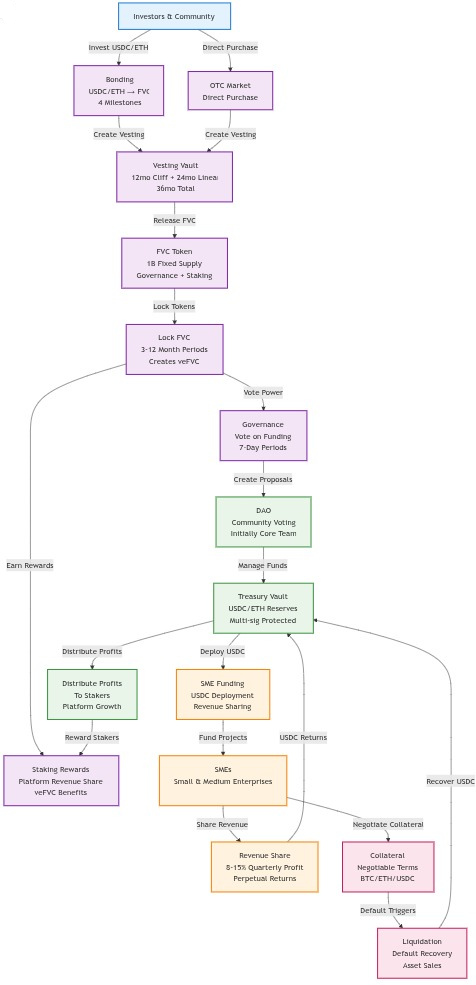
\includegraphics[keepaspectratio]{images/ecosystem.png}}
%\caption{FVC Ecosystem Architecture}
%\end{figure}
%%%
\subsection{5.5 Security Measures}\label{security-measures}

\begin{itemize}
\tightlist
\item
  \textbf{Multi-Signature Security}

  \begin{itemize}
  \tightlist
  \item
    \textbf{Multi-signature wallets} requiring 3 out of 5 authorised
    signers (founders) to approve any transaction
  \item
    \textbf{Treasury operations} protected by Gnosis Safe implementation
    with role-based access control
  \item
    \textbf{Emergency functions} require consensus among guardian
    signers
  \end{itemize}
\item
  \textbf{Timelock Implementation}

  \begin{itemize}
  \tightlist
  \item
    \textbf{Timelock delay} of 48 hours between governance proposal
    approval and execution
  \item
    \textbf{Gives token holders time to react} if they disagree with
    decisions or identify security concerns
  \item
    \textbf{Variable delays} based on operation criticality (7 days for
    critical operations)
  \item
    \textbf{Maximum delay cap} of 30 days for complex multi-step
    operations
  \end{itemize}
\item
  \textbf{Guardian Powers}

  \begin{itemize}
  \tightlist
  \item
    \textbf{Special emergency functions} that can immediately stop
    system functions during crises
  \item
    \textbf{Can pause/unpause smart contracts} to prevent exploits
  \item
    \textbf{Funds cannot be moved} during emergency pauses
  \item
    \textbf{Governance can be bypassed} during emergency situations
  \item
    \textbf{3-of-5 multisig controls this mechanism}
  \end{itemize}
\end{itemize}

\subsection{5.6 Upgrade Mechanisms}\label{upgrade-mechanisms}

\begin{itemize}
\tightlist
\item
  \textbf{UUPS Proxy Implementation}
\end{itemize}

The ecosystem implements OpenZeppelin's UUPS (Universal Upgradeable Proxy
Standard), a smart contract design pattern that allows developers to
upgrade contract logic while preserving the contract's address, state
and user balances. It works by delegating function calls to a nested
module within a contract, while FVC.sol contains a permanent address
users interact with, the actual logic is delegated to another
implementation which is upgradeable, changing nothing from the user's
perspective.

\subsection{5.7 Integration Architecture: How You Connect with Borrower
Systems}\label{integration-architecture-how-you-connect-with-borrower-systems}

\begin{itemize}
\tightlist
\item
  \textbf{External API Integration}
\end{itemize}

The system connects with established financial and legal infrastructure
through secure API integrations. Ondato provides KYC/AML verification
services with real-time status updates. DocuSign enables automated legal
document management and digital signature collection. Banking APIs
facilitate traditional payment processing and account verification for
SME borrowers.

All external integrations implement proper authentication, rate
limiting, and error handling to ensure reliable operation. Fallback
mechanisms and manual processing capabilities provide continuity during
external service disruptions.

\begin{itemize}
\tightlist
\item
  \textbf{Oracle Integration Framework}
\end{itemize}

The ecosystem integrates with multiple oracle systems for critical data
feeds. Chainlink price oracles provide real-time FVC/USD pricing for
bonding calculations and treasury management. Custom KYC compliance
oracles connect with external identity verification providers, enabling
automated eligibility verification while maintaining user privacy.

Oracle integration includes redundancy and validation mechanisms to
prevent manipulation or single points of failure. Price feeds implement
staleness checks and circuit breakers to halt operations during oracle
failures. KYC oracles utilise cryptographic attestations and
multi-provider verification for enhanced security.

\begin{itemize}
\tightlist
\item
  \textbf{Borrower System Integration}
\end{itemize}

The ecosystem connects with SME borrowers through standardised
revenue-sharing contract interfaces, enabling automated payment
processing and transparent revenue distribution. Borrowers deploy
ecosystem-compliant contracts that handle payment schedules, late fee
calculations, and automatic revenue forwarding to the ecosystem treasury.

The integration system supports multiple payment methods including
direct cryptocurrency transfers, traditional bank integration through
Plaid/Yodlee APIs, and manual payment processing for complex
arrangements. All payments are tracked on-chain with immutable records
for audit and compliance purposes.

\subsection{5.8 Data Architecture: On-Chain vs Off-Chain Data
Strategy}\label{data-architecture-on-chain-vs-off-chain-data-strategy}

\begin{itemize}
\tightlist
\item
  \textbf{On-Chain Data Strategy}
\end{itemize}

Critical ecosystem data including token balances, governance votes,
vesting schedules, and parameter configurations are stored directly on
the blockchain, ensuring immutability, transparency, and decentralised
access. Smart contracts emit comprehensive events for all state changes,
enabling efficient indexing and real-time monitoring.

On-chain storage optimisation reduces gas costs through packed data
structures, efficient storage layouts, and event-based rather than
storage-based logging where appropriate. The system prioritises data
integrity and accessibility while managing storage costs through careful
architectural decisions.

\begin{itemize}
\tightlist
\item
  \textbf{Off-Chain Data Management}
\end{itemize}

Privacy-sensitive information including KYC documents, legal agreements,
and business plans are stored off-chain using the InterPlanetary File
System (IPFS) for decentralised document storage. Documents are
encrypted where necessary and referenced on-chain through immutable
content hashes, ensuring integrity while maintaining privacy compliance.

The off-chain storage strategy includes redundancy through multiple IPFS
pinning services, automated backup procedures, and document lifecycle
management. Access controls ensure that sensitive documents are only
available to authorised parties while maintaining transparency for
public information.

\subsection{5.9 Tooling Stack}\label{tooling-stack}

\begin{itemize}
\tightlist
\item
  \textbf{Hardhat:} Full-stack Ethereum development environment for
  compiling, testing, deploying, and upgrading Solidity contracts.
\item
  \textbf{OpenZeppelin:} Secure libraries used for implementing ERC20,
  access control, and upgradeability via proxy patterns.
\item
  \textbf{Node.js \& npm:} JavaScript runtime (v18+ LTS recommended)
  with npm for dependency management and script execution.
\item
  \textbf{TypeChain:} Generates type-safe TypeScript bindings from
  contract ABIs for use in both backend and frontend layers.
\item
  \textbf{wagmi \& viem:} TypeScript-native libraries for wallet
  connections and contract interactions in React-based dApps.
\end{itemize}

\section{6. Pricing Strategy \& Presale Architecture}\label{dual-channel-presale-architecture}

\subsection{6.1 Presale Overview}\label{presale-overview}

Pre-listing capital is raised across two structured rounds: a tranched Seed Round for institutional investors and a six-tier backloaded Public Presale for the community. All prices denominated against the locked \$50M listing FDV (\$0.0500/token).

\begin{center}
\textbf{\$8.93M} Total Raise \quad | \quad \textbf{\$0.0290} Seed Avg \quad | \quad \textbf{\$0.0402} Presale Avg \quad | \quad \textbf{25\%} Pre-List Dilution
\end{center}

\subsection{6.2 Seed Round (Tranched)}\label{seed-round-tranched}

\begin{center}
\begin{tabular}{lcccc}
\toprule
\textbf{Tranche} & \textbf{Tokens} & \textbf{Price} & \textbf{Discount vs Listing} & \textbf{Capital Raised} \\
\midrule
Lead & 30M & \$0.0250 & 50\% & \$750K \\
Standard & 50M & \$0.0300 & 40\% & \$1,500K \\
Late & 20M & \$0.0325 & 35\% & \$650K \\
\midrule
\textbf{Seed Total} & \textbf{100M} & \textbf{\$0.0290 avg} & \textbf{42\% avg} & \textbf{\$2,900K} \\
\bottomrule
\end{tabular}
\end{center}

\textbf{Vesting:} 0\% TGE, 12-month cliff from payment (nothing claimable before TGE+3 months), 24-month linear vesting

\subsection{6.3 Public Presale (Six-Tier)}\label{public-presale-six-tier}

\begin{center}
\begin{tabular}{lcccc}
\toprule
\textbf{Tier} & \textbf{Tokens} & \textbf{Price} & \textbf{Discount vs Listing} & \textbf{Capital Raised} \\
\midrule
Tier 1 & 10M & \$0.0370 & 26\% & \$370K \\
Tier 2 & 18M & \$0.0380 & 24\% & \$684K \\
Tier 3 & 25M & \$0.0390 & 22\% & \$975K \\
Tier 4 & 32M & \$0.0400 & 20\% & \$1,280K \\
Tier 5 & 33M & \$0.0410 & 18\% & \$1,353K \\
Tier 6 & 32M & \$0.0426875 & 15\% & \$1,366K \\
\midrule
\textbf{Presale Total} & \textbf{150M} & \textbf{\$0.0402 avg} & \textbf{20\% avg} & \textbf{\$6,028K} \\
\bottomrule
\end{tabular}
\end{center}

\textbf{Vesting:} 0\% TGE, 6-month cliff, 12-month linear vesting (fully vested Month 18), with a partial instalment at M6

Presale Tier 1 at \$0.0370 sits above Seed Late at \$0.0325, so price and liquidity terms match round seniority. Average presale discount of about 20\% sits in the 18--25\% industry band. Combined raise: \$8,928,000.

\subsection{6.4 Use of Funds}\label{use-of-funds}

\begin{center}
\begin{tabular}{lccl}
\toprule
\textbf{Category} & \textbf{Amount} & \textbf{\% of Raise} & \textbf{Rationale} \\
\midrule
Business funding pool & \$3,928K & 44\% & Capital deployed into SME financing \\
DEX liquidity & \$1,161K & 13\% & Launch pool paired at listing price \\
Operating runway & \$893K & 10\% & About 26 months of core burn \\
Legal, compliance \& Shariah & \$536K & 6\% & BVI entity, opinions, SAFTs, scholar certification \\
Engineering, audits \& security & \$536K & 6\% & Audits, external build, infrastructure, bug bounty \\
Market making (wakala) & \$446K & 5\% & Agency fee plus quote-currency inventory \\
Exchange listings & \$446K & 5\% & Tier-2 CEX listing fees (negotiable) \\
Contingency & \$357K & 4\% & Unallocated reserve \\
Marketing \& KOLs & \$357K & 4\% & Community growth and campaigns \\
Lending entity \& regulatory & \$268K & 3\% & Entity contracting with SMEs \\
\bottomrule
\end{tabular}
\end{center}

\subsection{6.5 Community Channel (Bonding Mechanism)}\label{community-channel-bonding-mechanism}

The pre-sale phase incorporates a bonding mechanism with milestone-based pricing and controlled token distribution. This approach ensures controlled access whilst maintaining transparent price discovery.

The pricing is programmed as a reverse Dutch auction where the price starts low and gets higher to reward early participants. The only caveat is the prices have milestones rather than a gradual increase.

\subsection{6.6 Private Channel (OTC Swap)}\label{private-channel-otc-swap}

Parallel private channel for accredited investors featuring fixed pricing, allowlist verification, and custom allocation limits. Provides negotiated terms for institutional participants.

\section{7. Comparable Analysis}\label{comparable-analysis}

FVC's tokenomics is calibrated against five DeFi credit comparables. All data verified through CoinGecko, CoinMarketCap, and project documentation.

\begin{center}
\begin{tabular}{lccccc}
\toprule
\textbf{Project} & \textbf{Supply} & \textbf{Team} & \textbf{Investors} & \textbf{Public Sale} & \textbf{Listed} \\
\midrule
Maple Finance & 10M & 25\% & 26\% & 5\% & Apr 2021 \\
Goldfinch & 114M & 28.4\% & 21.6\% & 0\% & Jan 2022 \\
Centrifuge & 400M & 29.2\% & 18.5\% & 10.3\% & Jul 2021 \\
Ondo Finance & 10B & 33\% & 12.9\% & 2\% & Jan 2024 \\
Clearpool & 1B & 15\% & 12.3\% & 0.4\% & Oct 2021 \\
\midrule
\textbf{FVC (target)} & \textbf{1B} & \textbf{25\%} & \textbf{10\%} & \textbf{15\%} & \textbf{Q3 2026} \\
\bottomrule
\end{tabular}
\end{center}

\subsection{7.1 Where FVC Sits in the Competitive Landscape}\label{competitive-landscape}

\begin{itemize}
\tightlist
\item
  \textbf{Team (25\%)}: Mid-range; matches Maple, below Centrifuge and Ondo, above Clearpool.
\item
  \textbf{Investors (10\%)}: Lowest in set, signalling founder discipline.
\item
  \textbf{Public sale (15\%)}: highest in set, a deliberate community-first choice (closest comparable: Centrifuge at 10.3\%).
\end{itemize}

\textbf{Strategic Positioning:} Low investor allocation, high public sale, staggered cliffs, and programmatic governance differentiate FVC from earlier-generation DeFi credit protocols where insider concentration drove subsequent token underperformance.

\subsection{7.2 Performance Benchmark \& Lessons}\label{performance-benchmark}

Of five comparables, four lost 90--99\% from their all-time high. Only Ondo retained meaningful value, supported by the RWA narrative and an 18-month global lockup at launch.

\begin{center}
\small
\begin{tabularx}{\textwidth}{Y Y Y}
\toprule
\textbf{Lesson} & \textbf{Evidence} & \textbf{FVC Response} \\
\midrule
Long lockups outperform & Ondo: 18mo lockup, 5yr team vest $\rightarrow$ best performer & 40-month team vest, 18mo cliff \\
Narrative alone is insufficient & All 4 declining tokens lost narrative within 12--18mo & Revenue model creates fundamental backing \\
Insider concentration $\rightarrow$ decline & Goldfinch/Centrifuge: $\sim$50\% insider $\rightarrow$ >90\% decline & FVC combined insiders = 35\% \\
Tier-1 listings drive step-changes & Each tier-1 listing produced 50--200\% price jumps & \$900K reserved for tier-1 within 18mo \\
\bottomrule
\end{tabularx}
\end{center}

\section{8. Scenario Analysis}\label{scenario-analysis}

Tokenomics stress-tested across three scenarios. Prices are derived from the revenue model, not asserted. Each scenario specifies revenue, which feeds buy-and-burn, which determines implied price against effective float.

\textbf{Starting price:} \$0.0500 per FVC, corresponding to a \$50M fully diluted valuation and an approximate \$3M circulating market cap at TGE (60M tokens in float). All scenario trajectories begin from this anchor.

\subsection{8.1 Macroeconomic Regime Mapping}\label{macro-regime}

\begin{center}
\small
\begin{tabularx}{\textwidth}{p{3.2cm} Y Y Y}
\toprule
\textbf{Factor} & \textbf{Bear} & \textbf{Base} & \textbf{Bull} \\
\midrule
BTC / crypto trend & Sustained decline, crypto winter & Sideways / modest growth & BTC breakout, risk-on macro \\
Altcoin sentiment & Risk-off, flight to stables & Selective rotation & Broad rally, new ATHs \\
DeFi / RWA narrative & Low interest, TVL declining & Steady institutional adoption & RWA wave, regulatory tailwinds \\
Liquidity & Tight, VC dry powder scarce & Normalising & Abundant, FOMO-driven inflows \\
\bottomrule
\end{tabularx}
\end{center}

\subsection{8.2 Scenario Parameters \& Derived Pricing}\label{scenario-parameters}

\begin{center}
\begin{tabular}{lccc}
\toprule
\textbf{Indicator} & \textbf{Bear} & \textbf{Base} & \textbf{Bull} \\
\midrule
Starting price & \$0.050 & \$0.050 & \$0.050 \\
Revenue M24 & \$50K/mo & \$200K/mo & \$600K/mo \\
Revenue M48 & \$150K/mo & \$500K/mo & \$2M/mo \\
Quarterly burn M24 & $\sim$\$37K & $\sim$\$150K & $\sim$\$450K \\
Quarterly burn M48 & $\sim$\$112K & $\sim$\$375K & $\sim$\$1.5M \\
Programmatic minting & $\sim$5\% of allocation & $\sim$20\% of allocation & $\sim$35\% of allocation \\
Effective float M24 & $\sim$290M & $\sim$340M & $\sim$380M \\
CEX progression & Tier-2 only & Tier-1 by M18 & Tier-1 by M9 \\
Partnerships (24mo) & 0 & 2 & 4+ \\
Staking participation M36 & 10\% & 20\% & 35\% \\
\midrule
Price M12 & \$0.025 & \$0.040 & \$0.085 \\
Price M24 & \$0.012 & \$0.045 & \$0.140 \\
Price M48 & \$0.006 & \$0.065 & \$0.350 \\
\midrule
\textbf{Multiple vs listing} & \textbf{0.12x} & \textbf{1.30x} & \textbf{7.0x} \\
\bottomrule
\end{tabular}
\end{center}

\subsection{8.3 Probability-Weighted Expected Return}\label{expected-return}

Assigning indicative probabilities allows computation of a weighted expected return. These weights reflect current macro positioning, team execution capacity, and RWA sector tailwinds.

\begin{center}
\begin{tabular}{lcccc}
\toprule
\textbf{Scenario} & \textbf{Probability} & \textbf{M48 Price} & \textbf{Multiple} & \textbf{Weighted Return} \\
\midrule
Bear & 20\% & \$0.006 & 0.12x & 0.024x \\
Base & 50\% & \$0.065 & 1.30x & 0.650x \\
Bull & 30\% & \$0.350 & 7.00x & 2.100x \\
\midrule
\textbf{Expected outcome} & \textbf{100\%} & & & \textbf{2.77x} \\
\bottomrule
\end{tabular}
\end{center}

\textbf{Probability-Weighted Return: 2.77x vs Listing Price}

Seed investors at \$0.029 avg see a weighted expected 4.8x. Presale Tier 1 at \$0.030 see 4.6x. These weights are subjective; investors should stress-test against their own macro outlook. The 20/50/30 split reflects a moderately constructive view on the 2026--2030 crypto cycle.

\subsection{8.4 Price Derivation Methodology}\label{price-derivation}

\begin{itemize}
\tightlist
\item
  \textbf{Bear M48 (\$0.006):} \$150K/mo revenue generating $\sim$\$112K quarterly burn against $\sim$310M circulating tokens, insufficient buy pressure to offset sell pressure from unlocked vesting in a risk-off market.
\item
  \textbf{Base M48 (\$0.065):} \$500K/mo revenue, \$375K quarterly burn, growing treasury NAV of $\sim$\$8M against 360M float. Market prices at $\sim$1.3x NAV with tier-1 exchange liquidity.
\item
  \textbf{Bull M48 (\$0.350):} \$2M/mo revenue, \$1.5M quarterly burn creating significant supply contraction, treasury NAV >\$25M, and narrative premium from RWA/DeFi-VC leadership.
\end{itemize}

\section{9. Revenue Model \& Price Transmission}\label{revenue-model}

Token price is a function of protocol revenue, treasury flows, and supply dynamics, not speculation. This section establishes the causal chain from business activity to token value.

\subsection{9.1 Revenue Sources}\label{revenue-sources}

\textbf{SME Funding Revenue:} FVC deploys capital to vetted SMEs as interest-free loans and grants. Revenue is generated through origination fees, success fees, and revenue-sharing arrangements with portfolio SMEs. As active grants grow, recurring revenue scales linearly.

\textbf{Strategic Treasury Returns:} Idle treasury capital is deployed into yield-generating positions (stablecoin lending, RWA instruments, and strategic co-investments), creating a baseline revenue floor independent of new SME deal flow.

\textbf{Fiat Repayment Rails (Veil):} FVC plans to integrate Veil to facilitate SME repayments in fiat. Repayments collected in fiat are converted to stablecoins and settled to the protocol's multi-signature treasury safe, from which distributions are deployed to stakers. This gives funded businesses a conventional payment experience while keeping settlement, custody, and distribution transparent and on-chain.

\subsection{9.2 Price Transmission: How Revenue Becomes Token Value}\label{price-transmission}

Protocol revenue reaches the token through two primary channels:

\textbf{Channel 1 (Buy-and-Burn):} A fixed percentage of quarterly net revenue purchases FVC on the open market and permanently burns it via the token \texttt{burn()} path. This creates recurring buy pressure proportional to revenue and reduces total supply. There is no separate Buy \& Burn token allocation; burns are funded from income, not from a pre-minted bucket.

\textbf{Channel 2 (Treasury Accumulation):} SME repayments flow directly into the FVC treasury. As the treasury grows, the ratio of treasury assets to circulating supply creates an implicit NAV floor that the market prices against.

\subsection{9.3 The Causal Chain}\label{causal-chain}

More SMEs funded $\rightarrow$ more fees collected $\rightarrow$ larger quarterly burn $\rightarrow$ fewer tokens in supply $\rightarrow$ higher NAV/token $\rightarrow$ higher market price $\rightarrow$ staking becomes attractive $\rightarrow$ float shrinks further $\rightarrow$ each dollar of new demand moves price more. This is mechanical, not speculative.

\begin{center}
\begin{tabular}{lll}
\toprule
\textbf{Stage} & \textbf{Mechanism} & \textbf{Token Impact} \\
\midrule
SMEs funded & Origination / success fees collected & Treasury grows \\
Revenue accumulates & Quarterly buy-and-burn executes & Buy pressure + supply reduction \\
Treasury grows & NAV per circulating token rises & Price floor rises \\
Price rises & Staking yields become attractive & Tokens locked, float shrinks \\
Float shrinks & Demand against constrained supply & Price appreciation compounds \\
\bottomrule
\end{tabular}
\end{center}

\textbf{Governed Supply as Active Price Lever:} 35\% of total supply (Ecosystem + Treasury) is governance-gated under a 7-day timelock and a 2\% annual release cap. In bear conditions, governance restricts releases to reduce sell pressure. In bull conditions, measured releases fund growth while demand absorbs additional supply.

\section{10. Execution Strategy \& Bear-Case Mitigation}\label{execution-strategy}

Tokenomics does not survive execution failures. Six controllable factors separate Bear from Base and Base from Bull. Each factor is linked to its specific token-price impact.

\begin{center}
\small
\begin{tabularx}{\textwidth}{p{3cm} Y Y}
\toprule
\textbf{Factor} & \textbf{Target \& Mechanism} & \textbf{Token Price Impact} \\
\midrule
1. Revenue execution & Target \$200K/mo by M15 (Base), \$500K+ by M24 (Bull). Each \$100K/mo $\rightarrow$ $\sim$\$75K quarterly burn. If lagging at M12: freeze programmatic minting, pivot to higher-yield SMEs. & At Base M24 (\$0.045, $\sim$340M float), \$150K burn removes $\sim$3.3M tokens/quarter, a 1\% compounding supply reduction. \\
\addlinespace
2. Tier-1 CEX listing & \$900K reserved. Target: M18 (Base) or M9 (Bull). Adds \$5--20M daily volume for mid-cap tokens. & 50--200\% step-change per tier-1 listing. Institutional order flow sustains volume. \\
\addlinespace
3. Strategic partnerships & DeFi, TradFi, RWA, Shariah-compliant networks. Target: 2 in 24mo (Base), 4+ (Bull). & 30--100\% sustained appreciation per partnership. Each adding \$50K/mo fees shifts trajectory. \\
\addlinespace
4. Community \& staking & 20K+ holders, 5K+ voters within 12mo. Staking 20\% M36 (Base), 35\% (Bull). & 20\% staking on $\sim$340M float locks $\sim$68M tokens, amplifying burn price impact. \\
\addlinespace
5. Narrative capture & DeFi-VC, RWA tokenisation, Shariah-compliant DeFi. \$1.5M budget targeted at narrative leadership. & Capturing one narrative creates outsized capital inflows vs cost. \\
\addlinespace
6. Tokenomics discipline & Honour vesting, execute burn on schedule, governance-gate every mint. & Any deviation $\rightarrow$ >80\% drawdown. Discipline is non-negotiable. \\
\bottomrule
\end{tabularx}
\end{center}

\subsection{10.1 Bear-Case Mitigation Playbook}\label{bear-case-mitigation}

\begin{center}
\small
\begin{tabularx}{\textwidth}{p{4.4cm} Y Y}
\toprule
\textbf{Trigger} & \textbf{Defensive Action} & \textbf{Token Effect} \\
\midrule
Revenue < \$100K/mo at M12 & Freeze non-essential programmatic minting & Float growth $\rightarrow$ near zero \\
Price < \$0.02 & Accelerate burn to 40\% of revenue & Increases direct buy pressure \\
Staking < 10\% at M18 & Boosted staking incentives from Ecosystem bucket & Locks supply, reduces selling \\
No tier-1 by M18 & Redirect \$200K to tier-2 market-making & Deepens liquidity, cuts volatility \\
Partnership pipeline stalled & Pivot to protocol-to-protocol integrations & Faster revenue via DeFi composability \\
Community growth stalling & Redirect grants to community builder incentives & Organic holder growth \\
\bottomrule
\end{tabularx}
\end{center}

The goal is survival, not prevention. In a genuine crypto winter, all assets decline. The objective is to preserve operational capacity, community trust, and treasury reserves to emerge positioned for the next cycle. Projects surviving bear markets with intact tokenomics historically see 5--20x recovery multiples.

\section{11. TGE Planning}\label{tge-planning}

The Token Generation Event is the most consequential operational moment in the FVC roadmap. Planning covers four phases.

\subsection{11.1 Phase 1: Pre-Launch (T-30 $\rightarrow$ T-0)}\label{tge-phase-1}

\begin{center}
\begin{tabular}{lll}
\toprule
\textbf{Workstream} & \textbf{Timeline} & \textbf{Gate} \\
\midrule
Smart contracts deployed \& audited & T-30 $\rightarrow$ T-14 & Audit clean \\
Token contract verified on Etherscan & T-14 $\rightarrow$ T-7 & Public verification \\
Liquidity pool seeded (\$800K + 50M FVC) & T-7 $\rightarrow$ T-1 & USDC + FVC paired \\
Tier-2 CEX listing agreements & T-21 $\rightarrow$ T-3 & Min. 3 CEXs confirmed \\
Marketing campaign live & T-30 onwards & KOL roster activated \\
Vesting contracts deployed & T-14 $\rightarrow$ T-3 & Verified on-chain \\
Compliance \& legal sign-off & T-7 $\rightarrow$ T-1 & Final letter received \\
\bottomrule
\end{tabular}
\end{center}

\subsection{11.2 Phase 2: Launch Day (T-0)}\label{tge-phase-2}

Six-hour staggered sequence to avoid liquidity shocks. All times UTC.

\begin{center}
\begin{tabular}{ll}
\toprule
\textbf{Time} & \textbf{Action} \\
\midrule
T+0:00 & Token contract live; vesting contracts begin counting \\
T+0:30 & DEX pool opened (\$800K USDC + 50M FVC at \$0.05) \\
T+1:00 & Tier-2 CEX deposits enabled (Gate, KuCoin, MEXC) \\
T+2:00 & CEX trading live \\
T+3:00 & Live trading announcement \\
T+4:00 & Liquidity monitoring; market-making if needed \\
T+24:00 & Day-1 dashboard: holders, TVL, volume \\
\bottomrule
\end{tabular}
\end{center}

\subsection{11.3 Phase 3: Stabilisation (T+1 $\rightarrow$ T+30)}\label{tge-phase-3}

DEX pool above \$1M TVL with market-maker on standby. Target 5,000+ holders by T+30. Staking opens at T+7 (15\% participation target). First grants deployed at T+14 with 1--2 pilot SMEs, initiating the revenue flywheel. Tier-1 CEX outreach begins T+14.

\subsection{11.4 Phase 4: Post-Launch Milestones}\label{tge-phase-4}

\begin{center}
\begin{tabular}{lll}
\toprule
\textbf{Milestone} & \textbf{Target} & \textbf{Revenue / Token Impact} \\
\midrule
First grant repaid & M3 & Proves model; treasury begins accumulating \\
10 active grants & M6 & \$50K+/mo $\rightarrow$ first meaningful burn \\
First partnership & M9 & Pipeline expansion; 30--100\% step-change \\
Tier-1 CEX listing & M12--18 & 50--200\% step-change; institutional flow \\
\$200K/mo revenue & M15 & Sustains Base; \$150K quarterly burn \\
Second partnership & M18 & Compounds momentum \\
\$500K/mo revenue & M24 & Unlocks Bull; \$375K quarterly burn \\
\bottomrule
\end{tabular}
\end{center}

\subsection{11.5 Launch Risk Management}\label{launch-risk-management}

\begin{center}
\small
\begin{tabularx}{\textwidth}{p{4.4cm} Y}
\toprule
\textbf{Risk} & \textbf{Mitigation} \\
\midrule
Day-1 presale dump & 6-month cliff, zero presale tokens at TGE \\
DEX liquidity shock & Pre-seeded pool + market-maker standby \\
CEX listing delays & 3 tier-2 confirmed; 4th as backup \\
Smart contract exploit & 2 independent audits; bug bounty from T+0 \\
Insider selling & No insider unlock until M12 (Seed) / M18 (Team) \\
\bottomrule
\end{tabularx}
\end{center}

\section{12. Grants System}\label{grants-system}

\subsection{12.1 Dual Grant System}\label{dual-grant-system}

FVC offers two grant categories designed to serve different
SME and startup stages and capital needs.
All grants are interest-free and structured to align incentives between
the ecosystem and funded projects.

\subsubsection{Small Grants}\label{small-grants}

Small grants provide fast, accessible funding for early-stage projects
through a founder-friendly structure. Borrowers deposit minimal
collateral in yield-bearing assets. Projects share a small percentage of
revenue over a fixed period, no interest, no predetermined returns,
just aligned incentives. Fast-track vetting ensures quick deployment for
hackathon winners, MVP development, and bridge funding. Collateral only
serves as fraud protection, never liquidated for revenue shortfalls.
This model beats traditional lending terms while generating sustainable
ecosystem returns through actual business performance rather than
interest.

\textbf{Structure:}

\begin{itemize}
\tightlist
\item
  \textbf{Amount:} \$25,000 - \$100,000
\item
  \textbf{Collateral Requirement:} 10-30\% put down in stable assets:
  BTC, ETH, USDC et cetera, helping to protect staked funds.
\item
  \textbf{Revenue Share:} A percentage of gross revenue for 18-24 months
\item
  \textbf{Approval:} Fast-track vetting (72 - 168 hours)
\item
  \textbf{Liquidation:} Only triggered by fraud, misuse of funds, or
  project abandonment
\end{itemize}

\subsubsection{12.1.2 Large Strategic Grants}\label{large-strategic-grants}

Large grants fund established firms through two models: revenue share
agreements that preserve founder equity, or direct token/equity
investments for strategic partnerships. Projects undergo community
vetting where FVC token holders evaluate team, technology, and market
fit. Selected projects access capital plus FVC's ecosystem of advisors
and community supporters. Revenue shares run for a fixed term or
perpetually, generating sustainable yield for stakers without dilution.
Token/equity returns flow to the treasury and stakers constantly and
upon exit. This dual approach supports projects whether they're seeking
non-dilutive capital or established projects offering strategic
allocations.

\textbf{Type A: Revenue Share Agreement}

\textbf{Structure:}

\begin{itemize}
\tightlist
\item
  \textbf{Amount:} \$100,000 - \$500,000+
\item
  \textbf{Duration:} Perpetual or a fixed term
\item
  \textbf{Revenue Share:} A percentage of monthly gross revenue
\item
  \textbf{Approval:} Community vote after comprehensive vetting
\item
  \textbf{Collateral:} None required
\end{itemize}

\textbf{Type B: Equity/Token Investment}

\textbf{Structure:}

\begin{itemize}
\tightlist
\item
  \textbf{Amount:} \$100,000 - \$500,000+
\item
  \textbf{Investment Type:} Direct equity or token allocation
\item
  \textbf{Ownership:} A fixed percentage depending on stage and amount
\item
  \textbf{Approval:} Community vote with enhanced due diligence and the
  same comprehensive vetting
\item
  \textbf{Rights:} Standard investor protections (pro-rata, information
  rights)
\end{itemize}

SMEs and funded firms remit an agreed share of revenues at fixed time periods. Treasury allocates these revenues to: staking yields, FVC reserves and to buy and burn FVC.

\subsubsection{12.1.3 The Vetting Advantage}\label{the-vetting-advantage}

Unlike pure DAOs where anyone can propose anything, FVC employs a
specialised team that filters applications first:

\begin{enumerate}
\def\labelenumi{\arabic{enumi}.}
\tightlist
\item
  SMEs and startups Apply → Professional
  pitch deck, revenue model, team background
\item
  Expert Review → Our team eliminates obvious failures (90\% filtered)
\item
  Due Diligence → Deep dive on the top 10\%
\item
  Community Vote → Only pre-vetted, high-quality projects reach token
  holders
\end{enumerate}

Token holders vote on winners, rather than wading through garbage.
Professional filtering + community wisdom = superior returns.

\subsubsection{How Funding Works}\label{how-funding-works}

Application → Vetting (1 week) → Community Vote (3 days) → Instant
Funding

\textbf{Smart Contract Deployment:}

\begin{itemize}
\tightlist
\item
  \textbf{Approved projects get custom revenue-sharing contracts}
\item
  \textbf{A percentage of all revenues flow back automatically}
\item
  \textbf{No trust required - code enforces the agreement}
\item
  \textbf{Forever returns from one-time investments}
\end{itemize}

\textbf{What Projects Receive:}

\begin{itemize}
\tightlist
\item
  \textbf{Stable assets directly to their wallets (e.g.~ETH, BTC, USDC)}
\item
  \textbf{Marketing support from our community}
\item
  \textbf{Follow-on funding priority}
\end{itemize}

Professional vetting eliminates 90\% of noise. Community governance
selects from curated excellence. Every funded project has passed both
institutional-grade diligence AND community approval. Higher success
rates, better returns, happier token holders.

\subsection{12.2 Compliance and
Verification}\label{compliance-and-verification}

FVC implements a comprehensive revenue verification system that
applies uniformly to all grant recipients, ensuring transparency and
accountability across the portfolio. By combining on-chain automation
with off-chain attestation, FVC maintains accurate revenue
tracking while minimising trust assumptions. This hybrid approach
enables verification of both crypto-native and traditional revenue
streams, creating a robust framework for sustainable revenue sharing.

Whitelist mechanism ties wallet address to a zero-knowledge proof
generated via Ondato KYC process, the approved KYC and identity
attestation provider. Periodic identity verification ensures AML
compliance and sector-specific eligibility. No alternative providers
accepted without governance proposal and approval. Quarterly legal
reviews mandated. Registry excludes gambling, meme coins, adult content,
and unlicensed finance.

FVC's verification team, led by our CFA Accountant specialising
in revenue analysis, actively monitors for revenue manipulation tactics
including restructuring schemes, related-party transactions, and
artificial revenue deferrals. This professional oversight ensures
revenue sharing captures genuine business performance, with any attempts
to game the system triggering immediate investigation and potential
default proceedings.

\subsubsection{12.2.1 Enforcement and
Punishments}\label{enforcement-and-punishments}

FVC enforces revenue reporting through progressive penalties
designed to maintain compliance while allowing for operational
realities. Monthly reports receive a 7-day grace period for late
submission, after which the issue is escalated to the compliance team.
Missing filings result in immediate suspension from ecosystem
benefits including additional funding, community support, and governance
participation. Material misrepresentation or persistent non-compliance
triggers formal default proceedings, with smart contracts automatically
calculating accrued obligations and initiating recovery processes. All
enforcement actions are transparent, with status updates published to
maintain accountability while giving struggling projects opportunity to
remedy before severe consequences.

\subsection{12.3 Vetting Process}\label{vetting-process}

Grant applications undergo two-stage evaluation to ensure quality while
preserving decentralised governance. FVC's specialised due diligence
team, comprising chartered accountants, technical analysts, and
industry veterans, assesses each project's financial health, revenue
authenticity, technical feasibility, and market viability. Only projects
meeting strict operational and financial criteria advance to community
voting, accompanied by comprehensive vetting reports. This combination
of professional diligence and community governance ensures informed
capital allocation decisions while significantly reducing default risk
across the portfolio.

\section{13. Governance}\label{governance-section}

\subsection{13.1 Overview}\label{overview}

The FVC ecosystem contains a sophisticated, multi-layered governance
system designed to balance community participation with operational
efficiency. Our governance framework draws inspiration from successful
DeFi protocols while introducing innovative mechanisms specifically
tailored for SME funding operations.

\subsection{13.2 Core Governance
Architecture}\label{core-governance-architecture}

\textbf{Governance Token}: \$FVC serves as the primary governance token
with a fixed supply of 1 billion tokens. Each \$FVC token represents
voting power in ecosystem decisions, with additional mechanisms to
prevent concentration of power.

\textbf{Quadratic Voting Implementation}: FVC employs quadratic
voting to ensure democratic participation while mitigating whale
dominance. Voting power is calculated as the square root of
staked/locked tokens, creating a more equitable distribution of
influence. The Cost of Influence ($C_I$) for a desired Vote Weight ($W_v$) increases exponentially:

\[
C_I = (W_v)^2
\]

Therefore, to double influence ($2W_v$), an entity must stake four times the capital ($4C_I$), making governance capture economically inefficient.

\[
\text{Voting Power} = \sqrt{\text{Staked Tokens}}
\]

\textbf{Voting Mechanisms: Quorum Requirements, Vote
Delegation}\label{voting-mechanisms-quorum-requirements-vote-delegation}

\begin{itemize}
\tightlist
\item
  \textbf{Quorum Requirements:} 10\% of current veFVC supply must
  participate for vote validity. This ensures meaningful community engagement; prevents low participation rates and allows for dynamic adjustment based on ecosystem maturity.

  \textbf{Vote Delegation System:}

  \begin{itemize}
  \tightlist
  \item
    \textbf{Delegate Selection:} Holders can delegate votes to trusted
    community representatives
  \item
    \textbf{Transparency:} Public profiles and voting records for all
    delegates
  \item
    \textbf{Accountability:} Performance tracking and community
    oversight
  \item
    \textbf{Institutional Support:} Professional governance management
    for large holders
  \end{itemize}
\item
  \textbf{Voting Power Distribution:}

  \begin{itemize}
  \tightlist
  \item
    \textbf{Quadratic Voting:} Natural reduction of whale influence
  \item
    \textbf{Staking Requirements:} Voting power tied to staked/locked
    tokens
  \item
    \textbf{Anti-Flash Loan:} 1-day delay prevents borrowed-power
    manipulation
  \end{itemize}
\end{itemize}

\subsection{13.3 Emergency Procedures: Circuit Breakers, Emergency
Pause}\label{emergency-procedures-circuit-breakers-emergency-pause}

\begin{itemize}
\tightlist
\item
  \textbf{Pause Guardian System:}

  \begin{itemize}
  \tightlist
  \item
    \textbf{Multi-signature wallet (3 of 5 signers) with emergency pause
    capabilities}
  \item
    \textbf{Scope:} Can pause bonding, staking, and treasury operations
  \item
    \textbf{Limitations:} Cannot access funds or bypass governance
    mechanisms
  \item
    \textbf{Cooldown:} 24-hour minimum between emergency pauses
  \item
    \textbf{Maximum Duration:} 7-day pause limit with governance review
  \end{itemize}
\item
  \textbf{Emergency Response Protocol:}

  \begin{itemize}
  \tightlist
  \item
    \textbf{Immediate Activation:} Pause capability for security
    incidents
  \item
    \textbf{Community Notification:} Alert within 1 hour of activation
  \item
    \textbf{Governance Review:} Community assessment within 24 hours
  \item
    \textbf{Recovery Process:} Automatic unpause after cooldown unless
    extended
  \end{itemize}
\item
  \textbf{On-Chain Circuit Breaker:}

  \begin{itemize}
  \tightlist
  \item
    An automated \textbf{Algorithmic Risk Management} tool that mechanically suspends protocol operations during extreme market volatility to protect asset backing.
  \item
    \textbf{Treasury Limits:} Daily and single transfer caps prevent
    excessive outflows
  \item
    \textbf{Parameter Bounds:} Hard limits on critical ecosystem
    parameters
  \item
    \textbf{Emergency Fund:} Dedicated resources for crisis response
  \end{itemize}
\end{itemize}

\subsection{13.4 Governance Attack Prevention: Anti-Manipulation
Measures}\label{governance-attack-prevention-anti-manipulation-measures}

\begin{itemize}
\tightlist
\item
  \textbf{Voting Power Protection:}

  \begin{itemize}
  \tightlist
  \item
    \textbf{Snapshot Mechanism:} Voting power measured at fixed block
    height
  \item
    \textbf{Anti-Flash Loan:} 1-day delay prevents borrowed-power
    manipulation
  \item
    \textbf{Quadratic Voting:} Naturally reduces whale influence
  \item
    \textbf{Staking Requirements:} Voting power tied to locked tokens
  \end{itemize}
\item
  \textbf{Identity Verification:}

  \begin{itemize}
  \tightlist
  \item
    \textbf{KYC Integration:} Ondato implementation for regulatory
    compliance
  \item
    \textbf{Whitelist Management:} Controlled access to bonding and
    governance
  \item
    \textbf{Delegate Disclosures:} Public profiles for all voting
    representatives
  \item
    \textbf{Reputation System:} Track record of successful proposals and
    voting
  \end{itemize}
\item
  \textbf{Technical Safeguards:}

  \begin{itemize}
  \tightlist
  \item
    \textbf{Reentrancy Protection:} Standard OpenZeppelin security
    patterns
  \item
    \textbf{Access Controls:} Role-based permissions for administrative
    functions
  \item
    \textbf{Event Logging:} Complete audit trail for all governance
    actions
  \item
    \textbf{Upgrade Controls:} All contract modifications require
    governance approval
  \end{itemize}
\end{itemize}

\section{14. Distribution
Infrastructure}\label{distribution-infrastructure}

\textbf{Smart Contract System}

\begin{itemize}
\tightlist
\item
  \textbf{VestingVault Contract:} Automated token distribution and
  vesting management
\item
  \textbf{Multi-Signature Control:} Treasury and guardian oversight
\item
  \textbf{Emergency Pause:} Ability to halt distribution in emergencies
\item
  \textbf{Audit Trail:} Complete on-chain record of all distributions
\end{itemize}

\textbf{Multi-Signature Treasury}

\begin{itemize}
\tightlist
\item
  \textbf{Gnosis Safe:} 3-of-5 multi-signature wallet
\item
  \textbf{Founder Signers:} 3 founding team members
\item
  \textbf{Advisor Signers:} 2 strategic advisors
\item
  \textbf{Transaction Requirements:} Minimum 3 signatures
\end{itemize}

\section{15. Market Making Strategy}\label{market-making-strategy}

\textbf{Initial Liquidity Provision}

\begin{itemize}
\tightlist
\item
  \textbf{DEX Pools:} Uniswap V3 (FVC/USDC), Uniswap V3 (FVC/WETH)
\item
  \textbf{Initial Liquidity:} \$800K USDC + 50,000,000 FVC at \$0.05
\item
  \textbf{Range Management:} Concentrated liquidity for capital
  efficiency
\item
  \textbf{CEX Budget:} \$900K reserved for Tier-1 CEX listings within 18 months
\end{itemize}

\textbf{Liquidity Mining Incentives}

\begin{itemize}
\tightlist
\item
  \textbf{Base Rewards:} Yield for FVC/USDC liquidity providers
\item
  \textbf{Tiered Structure:} Higher rewards for longer-term provision
\item
  \textbf{Performance Metrics:} Volume and retention-based bonuses
\end{itemize}

\section{16. Risks and Mitigations}\label{risks-and-mitigations}

\subsection{16.1 Purpose}\label{purpose}

The purpose of this Risk Management Policy is to establish a structured
framework for identifying, assessing, mitigating, and monitoring risks
associated with FVC providing funding to SMEs and startups in the cryptocurrency and blockchain
industry. This policy ensures that FVC Asset Group Ltd.~operates in line
with industry best practices, regulatory expectations, and
Shariah-compliant financing principles.

\subsection{16.2 Due Diligence}\label{due-diligence}

The FVC Team evaluates grant applicants across multiple risk dimensions
before advancing projects to community vote. Our systematic approach
ensures only financially stable, technically sound, and credibly led
projects receive funding, protecting ecosystem resources while
maintaining high quality standards.

\textbf{Core Requirements:}

\begin{itemize}
\tightlist
\item
  \textbf{Financial Health:} Minimum 6-12 months runway demonstrated
  through bank statements and financial projections
\item
  \textbf{Team Verification:} Comprehensive background checks on all
  founders and directors including KYC, credit history, and reputational
  assessment
\item
  \textbf{Technical Assessment:} Code review, architecture evaluation,
  and security audit status for technical projects
\item
  \textbf{Risk Scoring:} Quantitative matrix evaluating financial
  stability, team credibility, technical soundness, and regulatory
  compliance
\item
  \textbf{Minimum Threshold:} Projects must achieve predetermined risk
  score across all categories to proceed to community voting
\end{itemize}

Projects failing any single criterion are rejected without exception,
ensuring consistent standards across the portfolio.

\subsection{16.3 Collateral and Security}\label{collateral-and-security}

FVC mitigates default risk through a robust collateral framework for
small grants, requiring borrowers to secure funding with digital assets
held in ecosystem-controlled smart contracts. This system provides
capital protection while maintaining transparent, automated enforcement
mechanisms that eliminate subjective decision-making in default
scenarios.

\textbf{Collateral Framework:}

\begin{itemize}
\tightlist
\item
  \textbf{Accepted Assets:} BTC, ETH, and stablecoins (USDC, USDT) held
  in multi-signature escrow contracts
\item
  \textbf{Collateralisation Ratio:} Tiered system depending on grant
  size and risk level. 10-30\% of grant value, with borrowers retaining
  staking yields
\item
  \textbf{Monitoring System:} Real-time mark-to-market valuation with
  automated alerts
\item
  \textbf{Margin Calls:} Triggered when collateral value falls below
  25\%, requiring top-up within 48 hours
\item
  \textbf{Liquidation Protocol:} Automatic liquidation upon three missed
  payments or collateral dropping below threshold
\item
  \textbf{Recovery Process:} Collateral sold to recover grant principal,
  excess returned to borrower
\end{itemize}

\subsection{16.4 Revenue}\label{revenue}

FVC structures repayments through revenue-sharing agreements rather than
interest-bearing loans, aligning ecosystem success with borrower growth
while eliminating fixed payment pressure during low-revenue periods.
Smart contract automation and transparent reporting requirements ensure
consistent revenue capture without relying on borrower goodwill.

\textbf{Revenue Structure:}

\begin{itemize}
\tightlist
\item
  \textbf{Sharing Model:} Fixed percentage of gross revenues rather than
  interest payments
\item
  \textbf{Payment Automation:} Smart contracts automatically route
  revenue shares from on-chain income
\item
  \textbf{Web3 Reporting:} Direct on-chain revenue verification through
  ecosystem integrations
\item
  \textbf{Traditional Business:} Monthly bank statement reconciliation;
  quarterly financial statements verified by chartered accountants as
  well as full annual audits
\item
  \textbf{Enforcement:} Three missed payments trigger default
  proceedings and collateral liquidation where applicable
\end{itemize}

This approach ensures sustainable repayment aligned with actual business
performance rather than arbitrary payment schedules.

\subsection{16.5 Treasury Concentration}\label{treasury-concentration}

FVC maintains strict concentration limits to ensure sustainable revenue
generation and minimise single-point-of-failure risks across the grant
portfolio. The treasury deploys capital across diverse sectors and
geographies, preventing overexposure to any single project, sector, or
regulatory jurisdiction.

\textbf{Concentration Limits:}

\begin{itemize}
\tightlist
\item
  \textbf{Per-Project Cap:} Capped amount of available treasury allocated
  to any single grant recipient. Subject to change
\item
  \textbf{Sector Diversification:} Grants distributed equally across
  varied sectors on-chain and off
\item
\textbf{Geographic Distribution:} Projects spanning multiple
jurisdictions to reduce regulatory concentration
\item
  \textbf{Revenue Source Variety:} Balance between established firms
  and emerging projects spanning Web2, Web3 and real world firms.
\item
  \textbf{Staged Deployment:} Initial grants limited to a smaller
  percentage of treasury, increasing only after successful repayment
  history
\end{itemize}

This disciplined approach to capital deployment ensures the ecosystem
maintains diverse revenue streams while protecting treasury resources
from concentrated default risk.

\subsection{16.6 Default and Insolvency}\label{default-and-insolvency}

When funded projects become insolvent or cease operations, FVC employs
multiple recovery mechanisms to minimise losses and protect treasury
resources. Our layered approach combines immediate collateral recovery
with longer-term asset claims, ensuring maximum value recovery while
maintaining transparent loss accounting for token holders.

\textbf{Recovery Mechanisms:}

\begin{itemize}
\tightlist
\item
  \textbf{Collateral Liquidation:} Immediate conversion of escrowed
  collateral to recover principal
\item
  \textbf{Asset Recovery Rights:} Contractual claims on intellectual
  property, token reserves, or equity stakes in parent entities
\item
  \textbf{Loss Buffer Reserve:} A percentage of treasury maintained in
  stablecoins to absorb expected defaults and aid in mitigating risk
\item
  \textbf{Transparent Write-Offs:} Losses recorded according to
  established accounting standards with public reporting
\end{itemize}

Default proceedings prioritise speed of recovery and capital
preservation, with recovered funds redistributed to active grants rather
than individual compensation.

\subsection{16.7 Counterparty and Compliance
Risk}\label{counterparty-and-compliance-risk}

FVC maintains strict compliance standards through comprehensive
KYC/AML procedures and continuous monitoring of all grant recipients.
This proactive approach prevents regulatory violations, protects the
ecosystem from sanctions exposure, and ensures all funded projects meet
international compliance standards.

\textbf{Compliance Framework:}

\begin{itemize}
\tightlist
\item
  \textbf{Identity Verification:} Mandatory KYC/AML checks including
  Ultimate Beneficial Owner (UBO) identification
\item
  \textbf{Blockchain Analytics:} Continuous monitoring transaction
  screening
\item
  \textbf{Ongoing Surveillance:} Real-time alerts for suspicious
  activity or regulatory changes
\item
  \textbf{Exclusion Criteria:} Automatic rejection of projects with
  sanctions exposure or regulatory violations
\item
  \textbf{Quarterly Reviews:} Regular compliance audits of all active
  grant recipients
\item
  \textbf{Geographic Restrictions:} Prohibited jurisdictions list
  maintained and updated monthly
\end{itemize}

\subsection{16.8 Regulation, Jurisdiction and Shariah
Compliancy}\label{regulation-and-shariah-compliancy}

FVC operates within established regulatory frameworks while
maintaining ethical finance principles through its revenue-sharing
model. The ecosystem's structure deliberately avoids interest-based
returns, aligning with both modern regulatory requirements and Islamic
finance principles through genuine risk-sharing arrangements.

\textbf{Jurisdictional Strategy:}

The project is legally structured in the British Virgin Islands (BVI)
based on specific legal counsel to mitigate Collective Investment
Scheme (CIS) risks within the United Kingdom. This offshore structuring
provides a robust legal foundation for the initial deployment phases.

\textbf{UK Regulatory Roadmap (2028-2029):}

FVC maintains active, provisional engagement with UK government
officials, including the Office of the Business Secretary. The
strategic roadmap targets the establishment of a fully regulated
exchange within the UK jurisdiction by 2028/29, contingent upon
financial stability milestones and the evolving UK crypto-asset
regulatory framework. This long-term vision aligns with growing UK
appetite for crypto-asset innovation and job creation.

\textbf{Compliance Measures:}

\begin{itemize}
\tightlist
\item
  \textbf{Regulatory Alignment:} Strategic BVI incorporation with
  roadmap for UK regulatory integration
\item
  \textbf{Revenue-Sharing Structure:} Interest-free model based on
  actual business performance rather than predetermined returns
\item
  \textbf{Shariah Principles:} Independent Shariah advisory panel to
  consistently ensure regulations are followed
\item
  \textbf{Legal Reviews:} Annual legal assessments to ensure continued
  compliance
\item
  \textbf{Transparent Reporting:} Public compliance updates and
  regulatory correspondence
\end{itemize}

This dual approach ensures broad accessibility while maintaining
regulatory compliance across jurisdictions.

\section{17. Exit \& Recovery Strategy}\label{exit-recovery-strategy}

\begin{itemize}
\tightlist
\item
  \textbf{Revenue-Based Exit:} Companies repay via revenue share until
  fixed term is reached or perpetually
\item
  \textbf{Equity Conversion:} In certain cases, revenue-sharing
  agreements may convert into equity
\item
  \textbf{Collateral Exit:} Default triggers automatic collateral
  liquidation
\item
  \textbf{Token Exit:} Token allocations received as part of agreements
  either liquidated or held as long-term treasury assets
\end{itemize}

% ── Back page ────────────────────────────────────────────────────────────────
\clearpage
\backgroundsetup{scale=1, angle=0, opacity=1, contents={}}
\thispagestyle{empty}
\begin{center}
  \vspace*{\fill}
  
\includegraphics[width=2.6cm]{images/fvc-logo.pdf}\par
  \vspace{1.1cm}
  \fvcgradientrule{0.28\textwidth}{1.2pt}\par
  \vspace{1.1cm}
  {\color{FVCInk}\large\bfseries FVC Asset Group Ltd\par}
  \vspace{0.4em}
  {\color{FVCGrey}\normalsize \href{https://fvcdigital.com}{fvcdigital.com}\, \textperiodcentered\, \href{mailto:info@fvcdigital.com}{info@fvcdigital.com}\par}
  \vspace*{\fill}
\end{center}

\end{document}

